\section{Macro Definition}
\label{group____useful__macro}\index{Macro Definition@{Macro Definition}}
the following macros will be used in the code of OCG  




Collaboration diagram for Macro Definition:\nopagebreak
\begin{figure}[H]
\begin{center}
\leavevmode
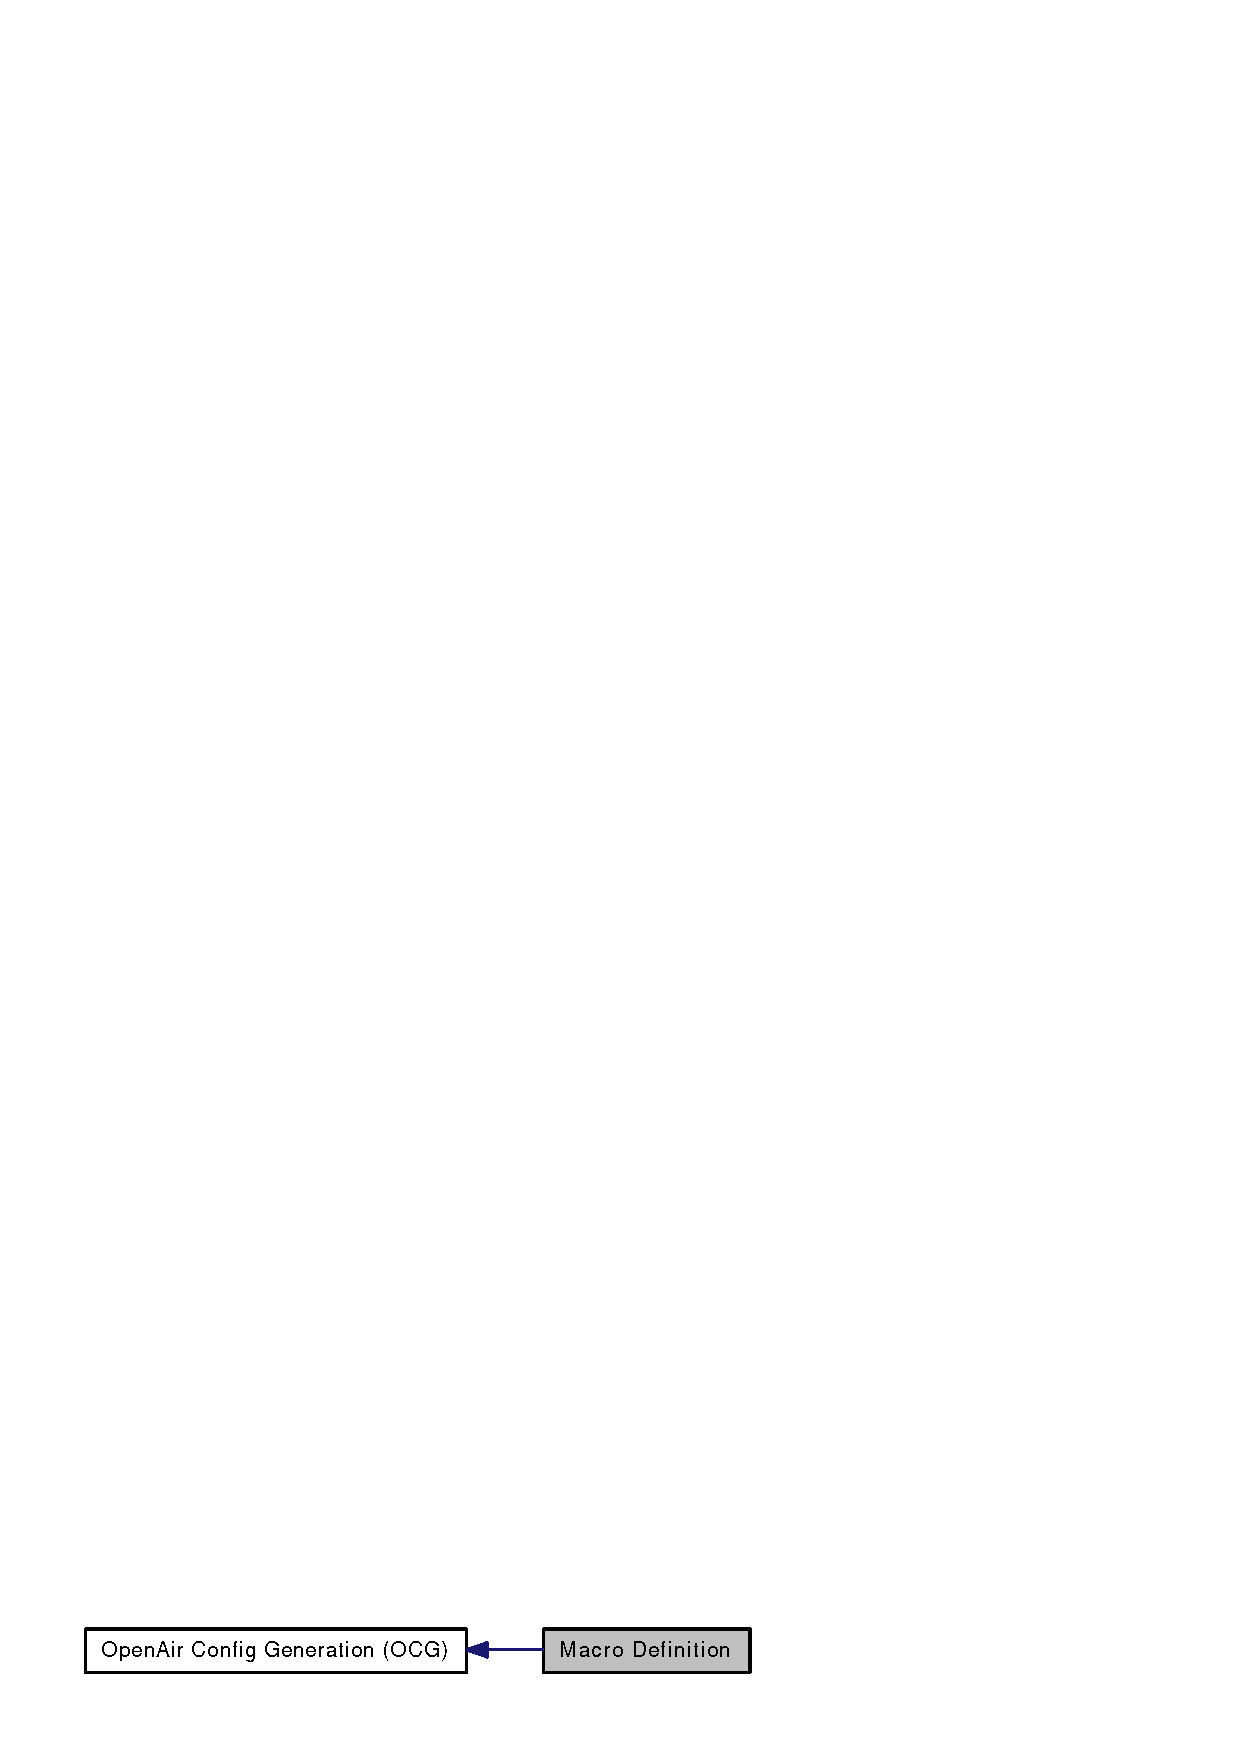
\includegraphics[width=182pt]{group____useful__macro}
\end{center}
\end{figure}
\subsection*{Defines}
\begin{CompactItemize}
\item 
\#define {\bf MODULE\_\-NOT\_\-PROCESSED}~-9999
\begin{CompactList}\small\item\em the module state indicator is set to -9999 before the module being processed \item\end{CompactList}\item 
\#define {\bf MODULE\_\-ERROR}~-1
\begin{CompactList}\small\item\em the module state indicator is set to -1 for error \item\end{CompactList}\item 
\#define {\bf MODULE\_\-OK}~0
\begin{CompactList}\small\item\em the module state indicator is set to 0 when successfully processed \item\end{CompactList}\item 
\#define {\bf GET\_\-HELP}~1
\begin{CompactList}\small\item\em the module state indicator is set to 1 for get\_\-opt\_\-OK when the user types -h option \item\end{CompactList}\item 
\#define {\bf NO\_\-FILE}~-2
\begin{CompactList}\small\item\em the module state indicator is set to -2 for detect\_\-file\_\-OK when no file is detected \item\end{CompactList}\item 
\#define {\bf WEB\_\-XML\_\-FOLDER}~\char`\"{}/nfs/webxml/\char`\"{}
\begin{CompactList}\small\item\em the web portal generates XML files into this folder \item\end{CompactList}\item 
\#define {\bf LOCAL\_\-XML\_\-FOLDER}~\char`\"{}local\_\-XML/\char`\"{}
\begin{CompactList}\small\item\em this folder contains some XML files for demo, users could also put their own XML files into this folder for a direct emulation without using the web portal \item\end{CompactList}\item 
\#define {\bf TEMP\_\-OUTPUT\_\-DIR}~\char`\"{}temp\_\-output/\char`\"{}
\begin{CompactList}\small\item\em temporary output files will be generated in this folder when folders for an emulation could not be created due to errors \item\end{CompactList}\item 
\#define {\bf OUTPUT\_\-DIR}~\char`\"{}/nfs/emu\_\-results/\char`\"{}
\begin{CompactList}\small\item\em this folder contains all the output files when folders for an emulation could be successfully created \item\end{CompactList}\item 
\#define {\bf FILENAME\_\-LENGTH\_\-MAX}~64
\begin{CompactList}\small\item\em the maximum length of a filename \item\end{CompactList}\item 
\#define {\bf DIR\_\-LENGTH\_\-MAX}~64
\begin{CompactList}\small\item\em the maximum length of the path name \item\end{CompactList}\item 
\#define {\bf MOBI\_\-XML\_\-FOLDER}~\char`\"{}mobi\_\-XML/\char`\"{}
\begin{CompactList}\small\item\em the folder that mobigen generate XML files in \item\end{CompactList}\item 
\#define {\bf DIR\_\-TO\_\-MOBIGEN}~\char`\"{}XML\_\-to\_\-mobigen/\char`\"{}
\begin{CompactList}\small\item\em the folder that mobigen detects XML file from OCG \item\end{CompactList}\end{CompactItemize}


\subsection{Detailed Description}
the following macros will be used in the code of OCG 

\subsection{Define Documentation}
\index{\_\-useful\_\-macro@{\_\-useful\_\-macro}!DIR\_\-LENGTH\_\-MAX@{DIR\_\-LENGTH\_\-MAX}}
\index{DIR\_\-LENGTH\_\-MAX@{DIR\_\-LENGTH\_\-MAX}!_useful_macro@{\_\-useful\_\-macro}}
\subsubsection[{DIR\_\-LENGTH\_\-MAX}]{\setlength{\rightskip}{0pt plus 5cm}\#define DIR\_\-LENGTH\_\-MAX~64}\label{group____useful__macro_g76232523706a1adf8f7e6b428912222b}


the maximum length of the path name 

\index{\_\-useful\_\-macro@{\_\-useful\_\-macro}!DIR\_\-TO\_\-MOBIGEN@{DIR\_\-TO\_\-MOBIGEN}}
\index{DIR\_\-TO\_\-MOBIGEN@{DIR\_\-TO\_\-MOBIGEN}!_useful_macro@{\_\-useful\_\-macro}}
\subsubsection[{DIR\_\-TO\_\-MOBIGEN}]{\setlength{\rightskip}{0pt plus 5cm}\#define DIR\_\-TO\_\-MOBIGEN~\char`\"{}XML\_\-to\_\-mobigen/\char`\"{}}\label{group____useful__macro_gba0dbe151f36dbb5a1e9d6a014a6e4bc}


the folder that mobigen detects XML file from OCG 

\index{\_\-useful\_\-macro@{\_\-useful\_\-macro}!FILENAME\_\-LENGTH\_\-MAX@{FILENAME\_\-LENGTH\_\-MAX}}
\index{FILENAME\_\-LENGTH\_\-MAX@{FILENAME\_\-LENGTH\_\-MAX}!_useful_macro@{\_\-useful\_\-macro}}
\subsubsection[{FILENAME\_\-LENGTH\_\-MAX}]{\setlength{\rightskip}{0pt plus 5cm}\#define FILENAME\_\-LENGTH\_\-MAX~64}\label{group____useful__macro_g367ba81f78d6fb6a2f0269fa891459ed}


the maximum length of a filename 

\index{\_\-useful\_\-macro@{\_\-useful\_\-macro}!GET\_\-HELP@{GET\_\-HELP}}
\index{GET\_\-HELP@{GET\_\-HELP}!_useful_macro@{\_\-useful\_\-macro}}
\subsubsection[{GET\_\-HELP}]{\setlength{\rightskip}{0pt plus 5cm}\#define GET\_\-HELP~1}\label{group____useful__macro_g2c856490debc47ae4f902edb5c866bcb}


the module state indicator is set to 1 for get\_\-opt\_\-OK when the user types -h option 

\index{\_\-useful\_\-macro@{\_\-useful\_\-macro}!LOCAL\_\-XML\_\-FOLDER@{LOCAL\_\-XML\_\-FOLDER}}
\index{LOCAL\_\-XML\_\-FOLDER@{LOCAL\_\-XML\_\-FOLDER}!_useful_macro@{\_\-useful\_\-macro}}
\subsubsection[{LOCAL\_\-XML\_\-FOLDER}]{\setlength{\rightskip}{0pt plus 5cm}\#define LOCAL\_\-XML\_\-FOLDER~\char`\"{}local\_\-XML/\char`\"{}}\label{group____useful__macro_ga29ecbb8fd7fe36832a39c0b91012af0}


this folder contains some XML files for demo, users could also put their own XML files into this folder for a direct emulation without using the web portal 

\index{\_\-useful\_\-macro@{\_\-useful\_\-macro}!MOBI\_\-XML\_\-FOLDER@{MOBI\_\-XML\_\-FOLDER}}
\index{MOBI\_\-XML\_\-FOLDER@{MOBI\_\-XML\_\-FOLDER}!_useful_macro@{\_\-useful\_\-macro}}
\subsubsection[{MOBI\_\-XML\_\-FOLDER}]{\setlength{\rightskip}{0pt plus 5cm}\#define MOBI\_\-XML\_\-FOLDER~\char`\"{}mobi\_\-XML/\char`\"{}}\label{group____useful__macro_g9faf2b41a72484a85c3562b70f15f874}


the folder that mobigen generate XML files in 

\index{\_\-useful\_\-macro@{\_\-useful\_\-macro}!MODULE\_\-ERROR@{MODULE\_\-ERROR}}
\index{MODULE\_\-ERROR@{MODULE\_\-ERROR}!_useful_macro@{\_\-useful\_\-macro}}
\subsubsection[{MODULE\_\-ERROR}]{\setlength{\rightskip}{0pt plus 5cm}\#define MODULE\_\-ERROR~-1}\label{group____useful__macro_g2a02efbd4b43aa3fa0b32d7acb954f14}


the module state indicator is set to -1 for error 

\index{\_\-useful\_\-macro@{\_\-useful\_\-macro}!MODULE\_\-NOT\_\-PROCESSED@{MODULE\_\-NOT\_\-PROCESSED}}
\index{MODULE\_\-NOT\_\-PROCESSED@{MODULE\_\-NOT\_\-PROCESSED}!_useful_macro@{\_\-useful\_\-macro}}
\subsubsection[{MODULE\_\-NOT\_\-PROCESSED}]{\setlength{\rightskip}{0pt plus 5cm}\#define MODULE\_\-NOT\_\-PROCESSED~-9999}\label{group____useful__macro_g3250a789f13c225a804d272b0b9674c8}


the module state indicator is set to -9999 before the module being processed 

\index{\_\-useful\_\-macro@{\_\-useful\_\-macro}!MODULE\_\-OK@{MODULE\_\-OK}}
\index{MODULE\_\-OK@{MODULE\_\-OK}!_useful_macro@{\_\-useful\_\-macro}}
\subsubsection[{MODULE\_\-OK}]{\setlength{\rightskip}{0pt plus 5cm}\#define MODULE\_\-OK~0}\label{group____useful__macro_g2035c06b028261848304fb79a02f6a99}


the module state indicator is set to 0 when successfully processed 

\index{\_\-useful\_\-macro@{\_\-useful\_\-macro}!NO\_\-FILE@{NO\_\-FILE}}
\index{NO\_\-FILE@{NO\_\-FILE}!_useful_macro@{\_\-useful\_\-macro}}
\subsubsection[{NO\_\-FILE}]{\setlength{\rightskip}{0pt plus 5cm}\#define NO\_\-FILE~-2}\label{group____useful__macro_g72e309f412bd15ef82fdba0eb5d1b056}


the module state indicator is set to -2 for detect\_\-file\_\-OK when no file is detected 

\index{\_\-useful\_\-macro@{\_\-useful\_\-macro}!OUTPUT\_\-DIR@{OUTPUT\_\-DIR}}
\index{OUTPUT\_\-DIR@{OUTPUT\_\-DIR}!_useful_macro@{\_\-useful\_\-macro}}
\subsubsection[{OUTPUT\_\-DIR}]{\setlength{\rightskip}{0pt plus 5cm}\#define OUTPUT\_\-DIR~\char`\"{}/nfs/emu\_\-results/\char`\"{}}\label{group____useful__macro_gdd836a505b86b88ac52e48d6bece5738}


this folder contains all the output files when folders for an emulation could be successfully created 

\index{\_\-useful\_\-macro@{\_\-useful\_\-macro}!TEMP\_\-OUTPUT\_\-DIR@{TEMP\_\-OUTPUT\_\-DIR}}
\index{TEMP\_\-OUTPUT\_\-DIR@{TEMP\_\-OUTPUT\_\-DIR}!_useful_macro@{\_\-useful\_\-macro}}
\subsubsection[{TEMP\_\-OUTPUT\_\-DIR}]{\setlength{\rightskip}{0pt plus 5cm}\#define TEMP\_\-OUTPUT\_\-DIR~\char`\"{}temp\_\-output/\char`\"{}}\label{group____useful__macro_g13d8f3ae0d419c0b5de8b1d746986952}


temporary output files will be generated in this folder when folders for an emulation could not be created due to errors 

\index{\_\-useful\_\-macro@{\_\-useful\_\-macro}!WEB\_\-XML\_\-FOLDER@{WEB\_\-XML\_\-FOLDER}}
\index{WEB\_\-XML\_\-FOLDER@{WEB\_\-XML\_\-FOLDER}!_useful_macro@{\_\-useful\_\-macro}}
\subsubsection[{WEB\_\-XML\_\-FOLDER}]{\setlength{\rightskip}{0pt plus 5cm}\#define WEB\_\-XML\_\-FOLDER~\char`\"{}/nfs/webxml/\char`\"{}}\label{group____useful__macro_g03306edded653a2fc4419653004d1f33}


the web portal generates XML files into this folder 

